%%%%%%%% ICML 2023 EXAMPLE LATEX SUBMISSION FILE %%%%%%%%%%%%%%%%%

\documentclass{article}

% Recommended, but optional, packages for figures and better typesetting:
\usepackage{microtype}
\usepackage{graphicx}
\usepackage{subfigure}
\usepackage{booktabs} % for professional tables


\usepackage{tikz}
% Corporate Design of the University of Tübingen
% Primary Colors
\definecolor{TUred}{RGB}{165,30,55}
\definecolor{TUgold}{RGB}{180,160,105}
\definecolor{TUdark}{RGB}{50,65,75}
\definecolor{TUgray}{RGB}{175,179,183}

% Secondary Colors
\definecolor{TUdarkblue}{RGB}{65,90,140}
\definecolor{TUblue}{RGB}{0,105,170}
\definecolor{TUlightblue}{RGB}{80,170,200}
\definecolor{TUlightgreen}{RGB}{130,185,160}
\definecolor{TUgreen}{RGB}{125,165,75}
\definecolor{TUdarkgreen}{RGB}{50,110,30}
\definecolor{TUocre}{RGB}{200,80,60}
\definecolor{TUviolet}{RGB}{175,110,150}
\definecolor{TUmauve}{RGB}{180,160,150}
\definecolor{TUbeige}{RGB}{215,180,105}
\definecolor{TUorange}{RGB}{210,150,0}
\definecolor{TUbrown}{RGB}{145,105,70}

% hyperref makes hyperlinks in the resulting PDF.
% If your build breaks (sometimes temporarily if a hyperlink spans a page)
% please comment out the following usepackage line and replace
% \usepackage{icml2023} with \usepackage[nohyperref]{icml2023} above.
\usepackage{hyperref}
\usepackage{caption}


% Attempt to make hyperref and algorithmic work together better:
\newcommand{\theHalgorithm}{\arabic{algorithm}}

\usepackage[accepted]{icml2023}

% For theorems and such
\usepackage{amsmath}
\usepackage{amssymb}
\usepackage{mathtools}
\usepackage{amsthm}

% if you use cleveref..
\usepackage[capitalize,noabbrev]{cleveref}

%%%%%%%%%%%%%%%%%%%%%%%%%%%%%%%%
% THEOREMS
%%%%%%%%%%%%%%%%%%%%%%%%%%%%%%%%
\theoremstyle{plain}
\newtheorem{theorem}{Theorem}[section]
\newtheorem{proposition}[theorem]{Proposition}
\newtheorem{lemma}[theorem]{Lemma}
\newtheorem{corollary}[theorem]{Corollary}
\theoremstyle{definition}
\newtheorem{definition}[theorem]{Definition}
\newtheorem{assumption}[theorem]{Assumption}
\theoremstyle{remark}
\newtheorem{remark}[theorem]{Remark}

% Todonotes is useful during development; simply uncomment the next line
%    and comment out the line below the next line to turn off comments
%\usepackage[disable,textsize=tiny]{todonotes}
\usepackage[textsize=tiny]{todonotes}


% The \icmltitle you define below is probably too long as a header.
% Therefore, a short form for the running title is supplied here:
\icmltitlerunning{Order in Chaos: Understanding Criminal Patterns in Germany}

\begin{document}

\twocolumn[
\icmltitle{Order in Chaos: Understanding Criminal Patterns in Germany}

% It is OKAY to include author information, even for blind
% submissions: the style file will automatically remove it for you
% unless you've provided the [accepted] option to the icml2023
% package.

% List of affiliations: The first argument should be a (short)
% identifier you will use later to specify author affiliations
% Academic affiliations should list Department, University, City, Region, Country
% Industry affiliations should list Company, City, Region, Country

% You can specify symbols, otherwise they are numbered in order.
% Ideally, you should not use this facility. Affiliations will be numbered
% in order of appearance and this is the preferred way.
\icmlsetsymbol{equal}{*}

\begin{icmlauthorlist}
\icmlauthor{Rojan Abolhassani}{equal,first}
\icmlauthor{Weronika Jaśkowiak}{equal,second}
\icmlauthor{Dóra Molnár}{equal,third}
\icmlauthor{Balázs Szabados}{equal,fourth}
\end{icmlauthorlist}

% fill in your matrikelnummer, email address, degree, for each group member
\icmlaffiliation{first}{Matrikelnummer 6665489, rojan.abolhassani@student.uni-tuebingen.de, MSc Machine Learning}
\icmlaffiliation{second}{Matrikelnummer 6761084, weronika.jaskowiak@student.uni-tuebingen.de, MSc Bioinformatics}
\icmlaffiliation{third}{Matrikelnummer 6728487, dora.molnar@student.uni-tuebingen.de, MSc Machine Learning}
\icmlaffiliation{fourth}{Matrikelnummer 6727211, balazs.szabados@student.uni-tuebingen.de, MSc Machine Learning}

% You may provide any keywords that you
% find helpful for describing your paper; these are used to populate
% the "keywords" metadata in the PDF but will not be shown in the document
\icmlkeywords{Machine Learning, ICML}

\vskip 0.3in
]

% this must go after the closing bracket ] following \twocolumn[ ...

% This command actually creates the footnote in the first column
% listing the affiliations and the copyright notice.
% The command takes one argument, which is text to display at the start of the footnote.
% The \icmlEqualContribution command is standard text for equal contribution.
% Remove it (just {}) if you do not need this facility.

%\printAffiliationsAndNotice{}  % leave blank if no need to mention equal contribution
\printAffiliationsAndNotice{\icmlEqualContribution} % otherwise use the standard text.

\begin{abstract}
Crime prevention and criminal justice are shared concerns in today's society,  driving the need for a comprehensive understanding of criminal patterns. In this project, we analyze \href{https://www.bka.de/EN/CurrentInformation/Statistics/PoliceCrimeStatistics/policecrimestatistics_node.html}{datasets} provided by the \textit{Bundeskriminalamt} containing police crime statistics from the years 2002-2022. Our analysis includes two approaches for predictions for future case numbers as well as gaining insight in the most frequent offences, the age distribution of suspects, and the tendencies in clearance rates throughout time. We aim to enhance understanding of underlying reasons and correlations using various statistical methods and visualizations.
\end{abstract}

\section{Introduction}\label{sec:intro}
In contemporary society, increasing concerns about crime prevention and upholding justice highlight the need for a deep understanding of criminal patterns. However, with numerous influencing factors, determining trends in criminal data is a considerable challenge. Our study focuses on police crime statistics from 2002 to 2022, aiming to extract key insights and forecast future number of offences.

During the analysis, we focused on two main approaches. In the first part, we elaborated on predicting the total number of offences for the upcoming years. We fitted various regression models \hyperref[subsec:methods_prediction]{(Section 3.1)} to the data spanning from 2002 to 2022. We compared the methods based on their error rates on randomly chosen test years. Additionally, we trained an autoregressive model to explore the time series perspective of the data \hyperref[subsec:methods_prediction]{(Section 3.1)}. The predictions from the two methods are detailed in \hyperref[subsec:results_pred]{Section 4.1}. In the second part we investigated two important aspects of criminal activity in Germany: age distribution among suspects \hyperref[subsec:methods_age]{(Section 3.2)} and effectiveness of the police (clearance rates) \hyperref[subsec:results_age]{(Section 4.2)}. The detailed results of our analysis and visualizations are included in \hyperref[sec:results]{Section 4}. In \hyperref[sec:conclusion]{Section 5} we present a sociological background that might have significantly influenced changes in criminal trends. All details of our work is also available on \href{https://github.com/rojan-abolhasani/Order-in-Chaos-Understanding-Criminal-Patterns-in-Germany}{GitHub}.




\section{Data}\label{sec:data}

For this project, we used multiple datasets consisting of PDF and Excel files from the \href{https://www.bka.de/EN/CurrentInformation/Statistics/PoliceCrimeStatistics/policecrimestatistics_node.html}{website of the \textit{Bundeskriminalamt}}, covering police crime statistics spanning from 2002 to 2022. Datasets from 2002 to 2013 are stored in PDF format and present a concise overview of crime trends. Among other features, they include the offence key, offence category name, number of recorded cases, change in the number of recorded cases compared to the previous year and clearance rates in percentage. We extracted this data into Excel files (Cases20**.xlsx).

Data between 2014 and 2022 are stored in Excel files and provide more detailed information. The data are organized into four tables: \\
\textbf{Cases Basic Table} - most importantly includes the offence key, offence category name, number of recorded cases, distribution of crime scenes grouped by the number of inhabitants in the area, clearance rate in percentage and the number of non-German suspects. \\
\textbf{Cases Development} - includes the offence key, offence category name, number of recorded cases, its change in percentage, and the clearance rate in percentage from the actual and previous year. \\
\textbf{Suspects} - provides information on suspects per offence, including their sex and age category.\\  
\textbf{Victims} - provides information on victims per offence, including their sex and age category.

%Additionally, we used \href{https://www.destatis.de/EN/Themes/Society-Environment/Population/Current-Population/Tables/lrbev02a.html}{population data} downloaded from the DeStatIs website.

The listed offences are assigned to keys. It is possible to distinguish main key groups based on characteristics shared by similar offences. For instance, the key '500000' correspond to offences related to property and forgery, but distinctions exist within this group: '530000' stands for misappropriation  and '540000' for document forgery. Within the main key groups, there are also smaller categories that aggregate specific types of offences.

Depending on the conducted analysis, we utilized both main key groups and more detailed ones related to specific types of crimes.

To grasp a first understanding of the data, \hyperref[fig:intro]{Figure 1} below provides an overview of the total number of cases, suspects, and victims from the examined years.

\begin{figure}[h]
    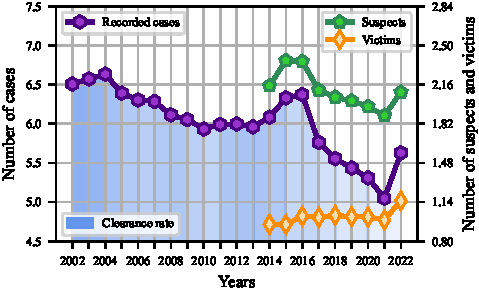
\includegraphics{introduction_plot.pdf}\label{fig:intro}
    \caption{The total number of recorded cases, suspects and victims each year in millions. The left y-axis represents recorded cases, while the right y-axis corresponds to both suspects and victims. The shading of each year's column indicates its average clearance rate, with darker colors representing lower rates and brighter colors reflecting higher rates. Note that all clearance rates fall within the range of 50-60\%.}
    
\end{figure}

\section{Methods}\label{sec:methods}

\subsection{Predicting total case numbers for the following years}\label{subsec:methods_prediction}
Our work involves two different approaches for predicting the total offence numbers in 2023 and beyond. Firstly, we fitted various regression models to the data between 2002 and 2022 using the Scikit-learn library of Python, including linear regression, kernel ridge regression, random forest regression, and decision tree regression. To assess the accuracy of these models, we randomly selected four test years and computed the $R^2$ and mean squared error on these data points. We also fitted polynomials with higher degrees to our data. Although the test errors of this method generally outperformed those of the previously mentioned models, it is not the most suitable technique for predicting the number of upcoming years, as further detailed later.

Building upon our regression analyses, we further explored the time series aspect of the dataset to forecast the total offence numbers for the next five years. We used an autoregressive model for our time series analysis. To address non-stationarity in the data, we applied first-order differencing. Influenced by an examination of the partial autocorrelation function, we chose an autoregressive component of order 5. The decision not to include a moving average component was based on insights from the autocorrelation function. We then trained and tested the model using the mean absolute percentage error, given the large scale of the total offences. Further results of these methods are discussed in \hyperref[subsec:results_pred]{Section 4.1}.

\subsection{Age distribution among suspects}\label{subsec:methods_age}

For the analysis of suspect age groups, we created a permutation test to determine whether the distribution of the number of suspects over the age groups is the same for males and females. 

We also attempted to examine if suspect ages are normally distributed through calculating its parameters and fitting different probability density functions to the data.


% This is the template for a figure from the original ICML submission pack. In lecture 10 we will discuss plotting in detail.
% Refer to this lecture on how to include figures in this text.
% 
% \begin{figure}[ht]
% \vskip 0.2in
% \begin{center}
% \centerline{\includegraphics[width=\columnwidth]{icml_numpapers}}
% \caption{Historical locations and number of accepted papers for International
% Machine Learning Conferences (ICML 1993 -- ICML 2008) and International
% Workshops on Machine Learning (ML 1988 -- ML 1992). At the time this figure was
% produced, the number of accepted papers for ICML 2008 was unknown and instead
% estimated.}
% \label{icml-historical}
% \end{center}
% \vskip -0.2in
% \end{figure}

\section{Results}\label{sec:results}

\subsection{Predicting total case numbers for the following years}\label{subsec:results_pred}
Due to the relatively small dataset, the performance of the fitted models varies significantly, mostly depending on the randomly chosen test years. Fitting polynomials with higher degrees usually resulted in lower error rates; however, due to the nature of these functions, they predict unrealistically high (or low) values for years outside the fitted region. Because of this, we continued our prediction with four models.  \begin{figure}[h!]\label{fig:prediction}
    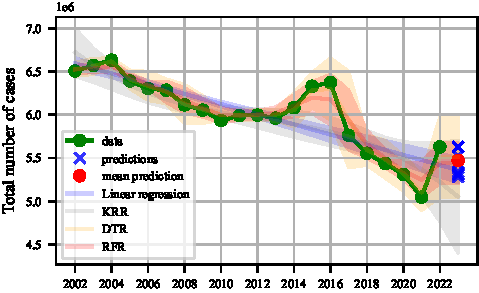
\includegraphics{prediction_models.pdf}
    \caption{Performance of linear regression, kernel ridge regression (KRR), decision tree regression (DTR) and random forest regression (RFR). For each method the standard deviation and the mean are visualized based on 10 rounds of training with 4 randomly chosen test years. The final prediction for 2023 is the mean of the 10 values given by the model with the least mean squared error in each round.}
    \label{fig:enter-label}
\end{figure}

Throughout the experiments, the best accuracy was achieved by the random forest and decision tree regressors. To obtain the final prediction for 2023, we fitted our models in 10 rounds and calculated the mean of the predictions given by the model with the lowest mean squared error in each round. The final prediction using this method was: 5,436,990.



Using the autoregressive model from \hyperref[subsec:methods_prediction]{Section 3.1}, the calculated error rate stands at 7.36\%, which, given the inherent variability in crime data, is relatively low. We then forecasted five steps ahead, spanning from 2023 to 2027, extending our analysis into the future. Specifically, our model predicts a total of 5,918,203 offences for the year 2023. Additionally, we complemented this analysis with \href{https://github.com/rojan-abolhasani/Order-in-Chaos-Understanding-Criminal-Patterns-in-Germany}{generated plots} that visually illustrate the steps of the method and the forecasted total numbers of offences for the specified period.

\subsection{Age distribution among suspects}



We formulated a hypothesis suggesting that the distribution of the number of suspects across age groups remains consistent between males and females. To test this hypothesis, we created a permutation test utilizing suspect data from the year 2022. The two samples for the test are the ages of male and female suspects. As the data only provides age groups and not exact ages, we generate the ages for the samples using the mean of each age group. In addition, we only use a thousandth of the suspects to be able to calculate a sufficient amount of permutations. As our test statistic, we chose the absolute difference of the sample means. Generating a million permutations, we obtained a p-value $\approx 0.155$. Since by calculating more permutations we can only increase this value, we retain our hypothesis.

Another assumption we had was that the age of suspects might be normally distributed. We suggested that choosing the mean around $37$ years, it would be reasonable to assume that it is equally likely that a suspect's age is $20$ or $54$ years. The following plot disproves this hypothesis: although the mean of the distribution is close to $37$, it initially grows quicker than the Gaussian with the parameters derived from the data and, as a result, decays more slowly.

\begin{figure}[h!]
    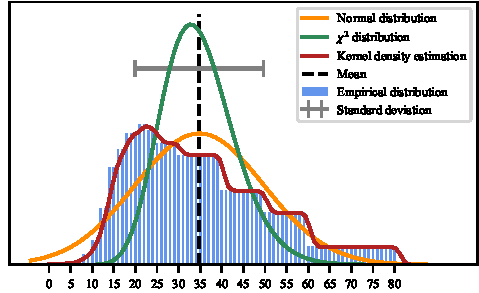
\includegraphics{age_group_distribution.pdf}
    \caption{The distribution of suspect ages. After calculating the mean and standard deviation of the empirical distribution, we plotted a Gaussian and a $\chi^2$ probability density function for comparison. Additionally, we computed a kernel density estimation.}
    \label{fig:enter-label}
\end{figure}


\subsection{Clearance rates}\label{subsec:results_age}
Clearance rate is one of the key metrics for assessing police efficiency. Based on the data, two important tendencies can be observed when looking at these percentages. Firstly, as shown in \hyperref[fig:intro]{Figure 1} and \hyperref[fig:clearance]{Figure 4}, the average rate of crimes solved by the police has an increasing value between the years 2002 and 2022. However, we have to note that the total number of offences shows a decreasing trend over the same period. Secondly, a strong correlation can be detected between the clearance rates and the types of crimes. \hyperref[fig:clearance]{Figure 4} visualizes this observation. We can see how offences in the category 'theft and burglary' have the lowest rates throughout the examined years while, for instance, the majority of 'offences against personal freedom' are solved by the police.

\begin{figure}[h!]
    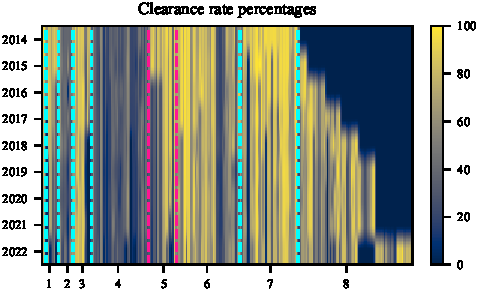
\includegraphics{clearance_rate_heatmap.pdf}
    \caption{The clearance rate percentage of offences each year. Each column represents a single offence. Dashed lines serve to group similar crimes together, white-collar crimes are highlighted with purple. $1:$ Offences against life and sexual self-determination, $2:$ Robbery, $3:$ Offences against personal freedom, $4:$ Theft and burglary, $5:$ White-collar crimes, $6:$ Other criminal offences, $7:$ Supplementary criminal laws, $8:$ Aggregate keys. In the last category many of the offences were not recorded in earlier years.}
    \label{fig:clearance}
\end{figure}

\subsection{Tendencies in the number of recorded crimes from 2002 to 2022}

The analysis of the total recorded cases revealed significant changes in separate periods, notably the highest number of recorded cases in 2004, followed by an increase in the years 2014-2015 compared to the previous years and a substantial decrease after 2016. A deeper insight into the data from 2004 and 2005 revealed that hostile sentiment among the public was on the rise, leading to the highest number of crimes in categories such as thefts, street crime, and fraud. The noticeable increase in 2014 and 2015 was especially prominent among non-German suspects (see \hyperref[fig:non-german]{Figure 5}), but we have to note that during this period, offences against foreigners are also at their highest across all years. After 2016, there is a monotonic decline in the number of recorded cases, which is only interrupted by the last recorded value. Some of the possible underlying reasons and influences are discussed in \hyperref[sec:conclusion]{Section 5}.

\begin{figure}[h!]
    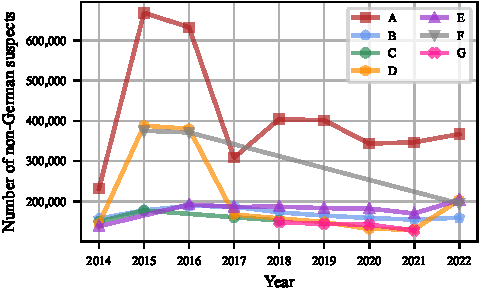
\includegraphics{top_5_offences_among_non_germans.pdf}
    \caption{Top 5 offences among non-German suspects in years 2014-2022. A: Unauthorised stay, B: Property and forgery offences, C: Total thefts, D: Offences against the Residence Act, the Asylum Act and the Freedom of Movement Act E.U., E: Offences involving brutality and crimes against personal freedom, F: Illegal entry, G: Bodily injury.}
    \label{fig:non-german}
\end{figure}


\section{Discussion \& Conclusion}\label{sec:conclusion}

In this project, we analyzed various datasets describing criminal activity in Germany between the years 2002 and 2022. Our work focused on predicting the total number of recorded cases for the upcoming years and examining different characteristics related to the recorded offences, such as the distribution of the age of suspects and the effectiveness of the police based on clearance rates. The main limitation of our work is the uncertainty surrounding the exact number of committed offences. Numerous factors may impact the willingness to report a crime, such as its severity and immediacy, the general trust in the work of the police, and the consequences of filing a report. Nevertheless, there are important societal-level influencing elements, including worldwide restrictions due to a pandemic \cite{covid_influence}. 

Lastly, it's important to highlight some key social, legal, and political events that could have had a significant impact on the changing number of recorded crimes from 2002 to 2022. Starting in 2004, an economic crisis occurred. The government, led by Chancellor Gerhard Schröder, implemented labor market reforms known as the 'Hartz reforms' between 2003 and 2005 \cite{financialcrisis, angrygermans}.  
In 2014 and 2015, Germany faced an unprecedented surge of asylum seekers and migrants, with a staggering influx of over 890,000 individuals into the country. At that time, Chancellor Angela Merkel declared that Germany would welcome refugees without imposing any legal limits \cite{sola,wassmer}. Between 2013 and 2017, German authorities underwent substantial legislative changes, particularly in the realm of criminal law. The goal was to address a spectrum of issues, including corruption in both public and private sectors, hate crimes, stalking, telecommunications interception, criminal asset confiscation, and corporate sanctions law \cite{wassmer}. In 2020, the outbreak of the global COVID-19 pandemic could have led to a decrease in the number of recorded cases \cite{covid_influence}. 

\section*{Contribution Statement}

Rojan Abolhassani made significant contributions to the prediction of case numbers and the analysis of clearance rates. Weronika Jaśkowiak focused on thoroughly examining various social aspects related to the dataset. Dóra Molnár played a role in data preparation, case number prediction, and the comprehensive analysis of clearance rates and age groups. Balázs Szabados actively participated in data preparation, conducted in-depth age group analysis, and contributed to the visualization of key insights. All team members conducted foundational data analysis and jointly co-authored this report.


\bibliography{bibliography}
\bibliographystyle{icml2023}




\end{document}


% This document was modified from the file originally made available by
% Pat Langley and Andrea Danyluk for ICML-2K. This version was created
% by Iain Murray in 2018, and modified by Alexandre Bouchard in
% 2019 and 2021 and by Csaba Szepesvari, Gang Niu and Sivan Sabato in 2022.
% Modified again in 2023 by Sivan Sabato and Jonathan Scarlett.
% Previous contributors include Dan Roy, Lise Getoor and Tobias
% Scheffer, which was slightly modified from the 2010 version by
% Thorsten Joachims & Johannes Fuernkranz, slightly modified from the
% 2009 version by Kiri Wagstaff and Sam Roweis's 2008 version, which is
% slightly modified from Prasad Tadepalli's 2007 version which is a
% lightly changed version of the previous year's version by Andrew
% Moore, which was in turn edited from those of Kristian Kersting and
% Codrina Lauth. Alex Smola contributed to the algorithmic style files.
